\chapter{Introdução}

O presente trabalho tem por objetivo apresentar os resultados e conclusões referentes ao projeto final da disciplina Identificação de Sistemas.

O trabalho consiste na análise de um sistema através do projeto de um filtro adaptativo \abbrev{FIR}{Finite Impulse Response} FIR (Finite Impulse Response). 

\section{Sistema utilizado}

O sistema utilizado é mostrado na \cref{fig:sistema}. 

\begin{figure}[!h]
	\centering
	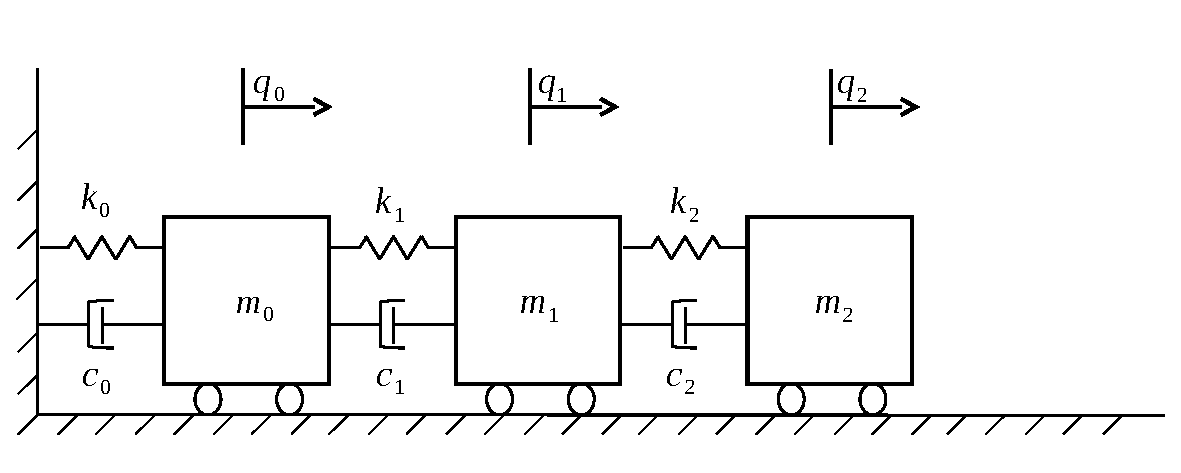
\includegraphics[width=0.8\textwidth]{IMGS/sistema.pdf}
	\caption{Sistema utilizado na análise.}
	\label{fig:sistema}
\end{figure}

Para este sistema temos que a energia cinética é:

\begin{equation}
T 
= \frac{1}{2}[m_0\dot{q_0}(t)^2 + m_1\dot{q_1}(t)^2 + m_2\dot{q_2}(t)^2] 
= \frac{1}{2}{\bf \dot{q}}^T(t)M{\bf \dot{q}}(t)
\end{equation}
onde 
\begin{equation*}
{\bf q(t)} = [q_0(t) \  q_1(t) \ q_2(t)]^T
\end{equation*}
é o vetor de configuração e
\begin{equation*}
M = 
\begin{bmatrix} 
m_0 & 0 & 0\\
0 & m_1 & 0 \\
0 & 0 & m_2
\end{bmatrix}
\end{equation*}  
é a matriz de massa do sistema.

A energia potencial tem a expressão:
\begin{equation}
\begin{split}
V &= \frac{1}{2}[k_0 q_0(t)^2 + k_1(q_1(t) - q_0(t))^2 + k_2 q_2(t)^2] \\
&= \frac{1}{2}[(k_0+k_1)q_0(t)^2 + (k_1+k_2)q_1(t)^2 + (k_2)q_2(t)^2 -2k_1  q_0(t)q_1(t) - 2k_2 q_2(t) \\
&= \frac{1}{2}{\bf \dot{q}}^T(t) K  {\bf \dot{q}}(t)
\end{split}
\end{equation}

onde
\begin{equation*}
K = 
\begin{bmatrix} 
k_0 +k_1 & -k_1 & 0\\
-k_1 & k_1+k_2 & -k_2 \\
0 & -k_2 & k_2
\end{bmatrix}
\end{equation*}   
é a matriz de rigidez do sistema.

Para o sistema utilizado temos que $m_i = 1 \ kg$ e $k_i = 1600 \ N/m$.

O amortecimento utilizado será o proporcional: $C = \alpha M + \beta K$. Iremos analisar o caso em que $\alpha = 10^{-3}$ e $\beta = 10^{-3}$.

\section{Resposta do sistema}

O sistema em questão possui a resposta \abbrev{FRF}{Função de Resposta em Frequência} FRF (Função de Resposta em Frequência) apresentada na \Cref{fig:FRF_all}

\begin{figure}[!h]
	\centering
	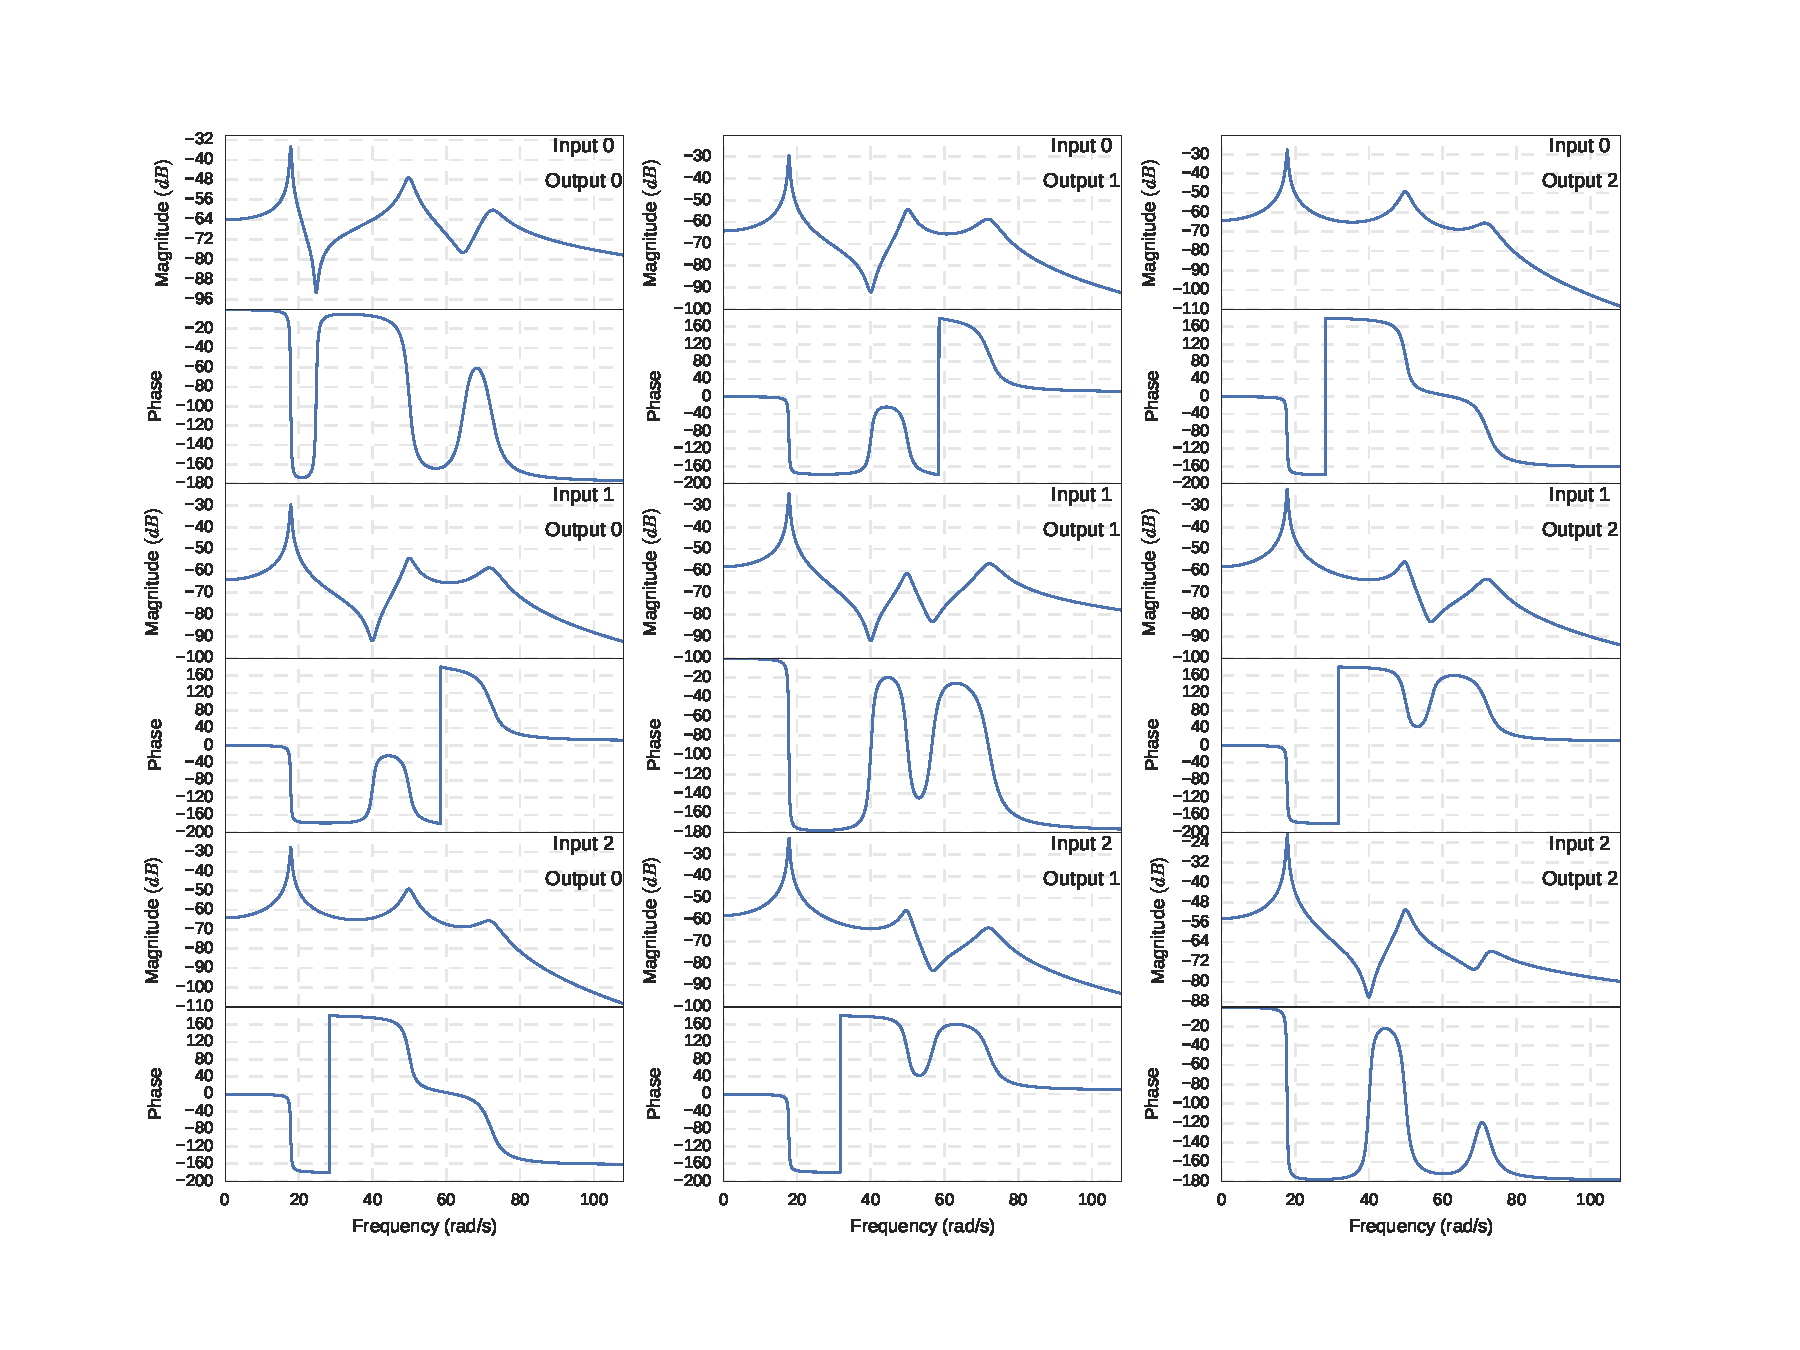
\includegraphics[trim={2.5cm, 2cm, 2.5cm, 2.5cm}, scale=0.6]{IMGS/FRF_all}
	\caption{FRF para o sistema em análise.}
	\label{fig:FRF_all}
\end{figure}

Para nossa análise iremos considerar uma força aplicada na massa 2 ($m_2$) e a medição nesta mesma massa, conforme ilustrado na \Cref{fig:sistemaf}. A aplicação da força nessa massa corresponde à FRF que pode ser visualizada no canto inferior direito (input=2 e output=2). A FRF em questão é também mostrada na \Cref{fig:FRF_i2_o2}

\begin{figure}
	\centering
	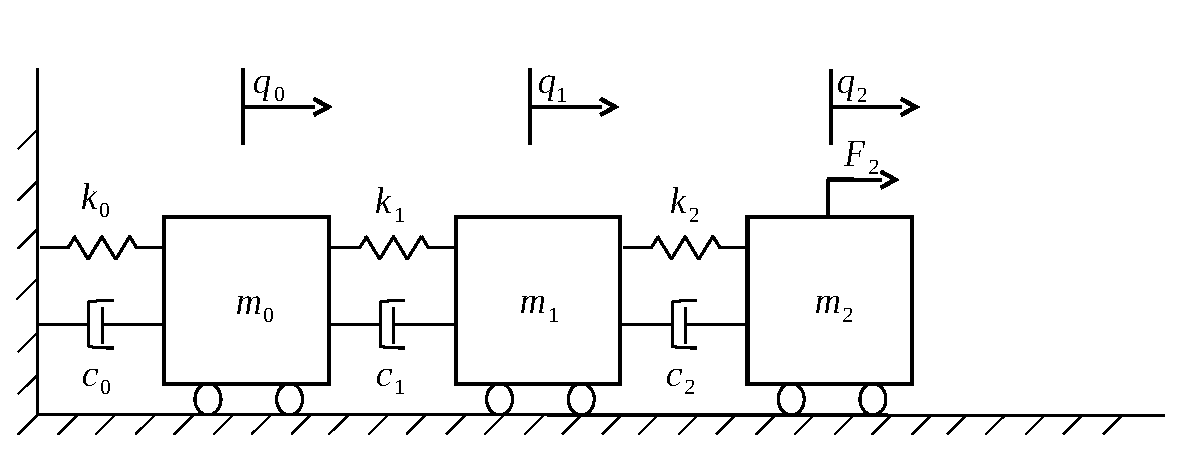
\includegraphics[width=0.8\textwidth]{IMGS/sistemaf}
	\caption{Aplicação de força e medição na massa $m_2$.}
	\label{fig:sistemaf}
\end{figure}

\begin{figure}
	\centering
	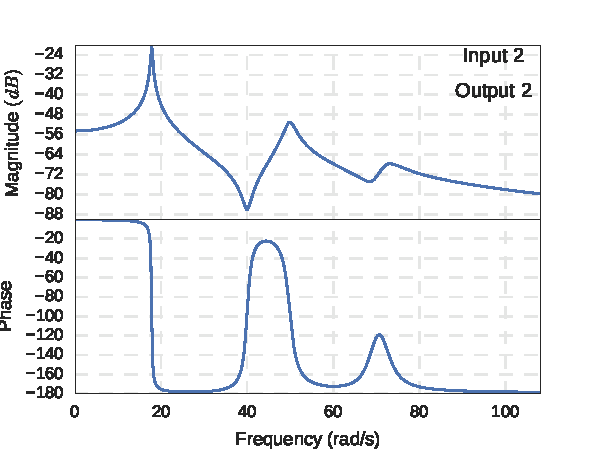
\includegraphics[scale=1]{IMGS/FRF_i2_o2}
	\caption{FRF para input em $m_2$ e medição em $m_2$.}
	\label{fig:FRF_i2_o2}
\end{figure}



